% \documentclass{} is the first command in any LaTeX code.  
% It is used to define what kind of document you are creating 
% such as an article or a book, and begins the document preamble
\documentclass{article} 

% Set the space between paragraphs
\setlength{\parskip}{1em}

% Packages for customizing the ToC
\usepackage{tocloft}
\usepackage{xcolor} % Package for color definitions
\usepackage{hyperref}

% Create trees
\usepackage{forest}

% Create two column content
\usepackage{multicol}

% Put blocks at their specific place using [H]
\usepackage{float}

\usepackage{algorithm}% http://ctan.org/pkg/algorithms
\usepackage{algpseudocode}% http://ctan.org/pkg/algorithmicx

\usepackage{amsmath}

% Create plots
\usepackage{pgfplots}
\pgfplotsset{compat=1.17}

% Use charts with axis that are strings instead of number
\usepackage{pgfplotstable}

% For better looking tables
\usepackage{booktabs} 

% Add dots to the table of contents
\renewcommand{\cftsecleader}{\cftdotfill{\cftdotsep}}
\renewcommand{\cftsubsecleader}{\cftdotfill{\cftdotsep}}
\renewcommand{\cftsubsubsecleader}{\cftdotfill{\cftdotsep}}

% Define custom colors using xcolor
\definecolor{green400}{HTML}{4ade80}
\definecolor{green500}{HTML}{22c55e}
\definecolor{green600}{HTML}{16a34a}
\definecolor{blue400}{HTML}{60a5fa}
\definecolor{blue500}{HTML}{3b82f6}
\definecolor{blue600}{HTML}{2563eb}
\definecolor{blue700}{HTML}{1d4ed8}
\definecolor{violet600}{HTML}{8b5cf6}
\definecolor{violet400}{HTML}{a78bfa}

% Hyperlink settings
\hypersetup{
    % Enable colored links
    colorlinks=true,
    % Color for internal links (sections, pages, etc.)
    linkcolor=blue700,
    % Color for external URLs
    urlcolor=blue600,
    % Color for citation links
    citecolor=blue700
}

% Bibliography package
\usepackage[backend=biber,style=numeric]{biblatex}
\addbibresource{references.bib}

% Article title
\title{LeanIMT: An optimized Incremental Merkle Tree} 
% Authors name
\author{Privacy \& Scaling Explorations} 
% Date for date compiled
\date{\today} 

% The preamble ends with the command \begin{document}
% All begin commands must be paired with an end command somewhere
\begin{document}
% Creates title using information in preamble (title, author, date)
\maketitle

% Creates a section for the Abstract
\section{Abstract}

\newpage
Created: \date{\today}

Updated: \date{\today}

% Insert a new page
\newpage
% Insert the Table of Contents
\tableofcontents
% Insert a new page
\newpage

% Creates a section for the Introduction
\section{Introduction}

% Creates a subsection for the Motivation within Introduction
\subsection{Motivation}

\section{Merkle Tree}

\subsection{Incremental Merkle Tree}

An Incrememental Merkle Tree (IMT) is a Merkle Tree (MT) designed to be updated efficiently.

% align to the left
\raggedright



\subsection{Binary Tree}

A Binary Tree is a tree data structure in which each node has at most two children, referred to as the left child and the right child.

TODO: Explain what is a Merkle tree and an Incremental Merkle Tree.

% Add a new empty line


% Generic Merkle Tree 

\begin{center}
    \begin{forest}
        for tree={edge path={\noexpand\path[\forestoption{edge}] (\forestOve{\forestove{@parent}}{name}.parent anchor) -- +(0,-18pt)-| (\forestove{name}.child anchor)\forestoption{edge label};}, rectangle, draw, align=center}
        [$H_6$ \\ \color{blue600}H($H_4{||}H_5$)
        [$H_4$ \\ \color{blue600}H($H_0{||}H_1$) [$H_0$ \\ \color{blue600}H($a_0{||}a_1$) [$a_0$] [$a_1$]] [$H_1$ \\ \color{blue600}H($a_2{||}a_3$) [$a_2$] [$a_3$]]]
        [$H_5$ \\ \color{blue600}H($H_2{||}H_3$) [$H_2$ \\ \color{blue600}H($a_4{||}a_5$) [$a_4$] [$a_5$]] [$H_3$ \\ \color{blue600}H($H_6{||}H_7$) [$a_6$] [$a_7$]]]
        ]
    \end{forest}
\end{center}



\section{LeanIMT}

\subsection{Definition}



The \textbf{LeanIMT} (Lean Incremental Merkle Tree) is a Binary IMT.



% align to the left
\raggedright

The LeanIMT has two properties:

1. Every node with two children is the hash of its two child nodes.

2. Every node with one child has the same value as its child node.

The tree is always built from the leaves to the root.

The tree will always be balanced by construction.

In a LeanIMT a node is either a leaf or a parent.



Example of a LeanIMT



$T$ - Tree

$V$ - Vertices (Nodes)

$E$ - Edges (Lines connecting Nodes)



$T = (V,E)$

% align to the left
\raggedright



$V = \{a_0, a_1, a_2, H_0, H_1, H_2\}$



$E = \{(a_0, H_0), (a_1, H_0), (a_2, a_2), (H_0, H_1), (a_2, a_2)\}$



\begin{center}
    \begin{forest}
        for tree={edge path={\noexpand\path[\forestoption{edge}] (\forestOve{\forestove{@parent}}{name}.parent anchor) -- +(0,-18pt)-| (\forestove{name}.child anchor)\forestoption{edge label};}, rectangle, draw, align=center}
        [$H_1$ \\ \color{blue600}H($H_0{||}a_2$)
        [$H_0$ \\ \color{blue600}H($a_0{||}a_1$)
        [$a_0$]
            [$a_1$]
        ]
        [$a_2$ \\ \color{blue600}$a_2$
        [$a_2$]
        ]
        ]
    \end{forest}
\end{center}



\subsection{Insertion}

There are two cases:

1. When the new node is a left node.

2. When the new node is a right node.



We will always see one of these cases in each level when we are inserting a node. It is like, when you insert a node, if that node is left node, the parent node which is in the next level, will be the same node. If it is a right node the parent node, will be the hash of this node with the node in its left. This algorithm will be the same in each level, not only in level 0.



\subsubsection*{Case 1: The new node is a left node}

It will not be hashed, it's value will be sent to the next level.



If we add $a_4$.



$T = (V,E)$

% align to the left
\raggedright



$V = \{a_0, a_1, a_2, a_3, H_0, H_1, H_2\}$



$E = \{(a_0, H_0), (a_1, H_0), (a_2, H_1), (a_3, H_1), (H_0, H_2), (H_1, H_2)\}$



% \vbox is used to group the diagrams next to each other
\vbox{
    \begin{multicols}{2}
        \vfill
        \columnbreak
        \vspace*{\fill}
        \begin{center}
            \begin{forest}
                for tree={edge path={\noexpand\path[\forestoption{edge}] (\forestOve{\forestove{@parent}}{name}.parent anchor) -- +(0,-12pt)-| (\forestove{name}.child anchor)\forestoption{edge label};}, rectangle, draw, align=center}
                [$H_2$
                [$H_0$
                        [$a_0$]
                            [$a_1$]
                    ]
                    [$H_1$
                        [$a_2$]
                            [$a_3$]
                    ]
                ]
            \end{forest}
        \end{center}
        \begin{center}
            \textit{Before inserting $a_4$}
        \end{center}
        \begin{center}
            \begin{forest}
                for tree={edge path={\noexpand\path[\forestoption{edge}] (\forestOve{\forestove{@parent}}{name}.parent anchor) -- +(0,-12pt)-| (\forestove{name}.child anchor)\forestoption{edge label};}, rectangle, draw, align=center}
                [$H_3$, draw=blue600, top color=blue600!0, bottom color=blue600!0, line width=1pt
                [
                $H_2$ [$H_0$ [$a_0$] [$a_1$]] [$H_1$ [$a_2$] [$a_3$]]
                ]
                [$a_4$ , edge={blue600, line width=1pt}, draw=blue600, top color=blue600!0, bottom color=blue600!0, line width=1pt [$a_4$ , edge={blue600, line width=1pt}, draw=blue600, top color=blue600!0, bottom color=blue600!0, line width=1pt [$a_4$ , edge={blue600, line width=1pt}, draw=blue600, top color=blue600!0, bottom color=blue600!0, line width=1pt]]]
                ]
            \end{forest}
        \end{center}
        \begin{center}
            \textit{After inserting $a_4$}
        \end{center}
    \end{multicols}
}



\subsubsection*{Case 2: The new node is a right node}



If we add $a_5$.



\vbox{
    \begin{multicols}{2}

        % Fill a space
        \vfill
        \columnbreak
        \vspace*{\fill}
        % Fill a space

        \begin{center}
            \begin{forest}
                for tree={edge path={\noexpand\path[\forestoption{edge}] (\forestOve{\forestove{@parent}}{name}.parent anchor) -- +(0,-12pt)-| (\forestove{name}.child anchor)\forestoption{edge label};}, rectangle, draw, align=center}
                [$H_3$
                [
                        $H_2$ [$H_0$ [$a_0$] [$a_1$]] [$H_1$ [$a_2$] [$a_3$]]
                    ]
                    [$a_4$ [$a_4$ [$a_4$]]]
                ]
            \end{forest}
        \end{center}
        \begin{center}
            \textit{Before inserting $a_5$}
        \end{center}
        % Fill a space
        \vfill
        \columnbreak
        \vspace*{\fill}
        % Fill a space
        \begin{center}
            \begin{forest}
                for tree={edge path={\noexpand\path[\forestoption{edge}] (\forestOve{\forestove{@parent}}{name}.parent anchor) -- +(0,-12pt)-| (\forestove{name}.child anchor)\forestoption{edge label};}, rectangle, draw, align=center}
                [$H_5$, draw=blue600, top color=blue600!0, bottom color=blue600!0, line width=1pt
                [
                $H_2$ [$H_0$ [$a_0$] [$a_1$]] [$H_1$ [$a_2$] [$a_3$]]
                ]
                [$H_4$ , edge={blue600, line width=1pt}, draw=blue600, top color=blue600!0, bottom color=blue600!0, line width=1pt [$H_4$ , edge={blue600, line width=1pt}, draw=blue600, top color=blue600!0, bottom color=blue600!0, line width=1pt [$a_4$] [$a_5$ , edge={blue600, line width=1pt}, draw=blue600, top color=blue600!0, bottom color=blue600!0, line width=1pt]]]
                ]
            \end{forest}
        \end{center}
        \begin{center}
            \textit{After inserting $a_5$}
        \end{center}
    \end{multicols}
}



\subsubsection{Pseudocode}

\begin{algorithm}[H]
    \caption{LeanIMT Insert algorithm}\label{insert}
    \begin{algorithmic}[1]
        \Procedure{Insert}{$leaf$}
        \If{$depth < newDepth$} \Comment{$newDepth$ is the new depth of the tree after inserting the new node}
        \State add a new empty array to nodes \Comment{Add a new tree level}
        \EndIf
        \State $node\gets leaf$
        \State $index\gets size$ \Comment{The index of the new leaf equals the number of leaves in the tree.}
        \For{level from 0 to depth - 1}
        \State nodes[level][index] $\gets$ node
        \If{index \textbf{is odd}} \Comment{It's a right node}
        \State sibling $\gets$ nodes[level][index - 1]
        \State node $\gets$ \textbf{hash}(sibling, node)
        \EndIf
        \State index $\gets$ $\lfloor index/2 \rfloor$ \Comment{Divides the index by 2 and discards the remainder.}
        \EndFor
        \State nodes[depth] $\gets$ [node] \Comment{Store the new root at the top level}
        \EndProcedure
    \end{algorithmic}
\end{algorithm}



\subsubsection{Correctness}

The idea is to prove that after inserting a new node to the LeanIMT, the tree keeps all the properties.

The Mathematical Induction method will be used to prove the correctness of the algorithm.

$n$: Number of leaves

$T$: LeanIMT Tree

$n=0$

If the tree is empty, the Insert function returns a new node with the value of the leaf. This satisfies the LeanIMT poperties because the node does not have children. (Trivial case)

$n \Rightarrow n+1$

Let's assume that with $n$ nodes, the tree T is a correct LeanIMT and prove that with $n+1$ nodes, T is still a correct LeanIMT. (Inductive step)

The new node is always added at the end of the list of nodes.

To insert a new node, there are two possible cases:

1. When the new node is a left node

2. When the new node is a right node

Case 1

If the new node is a left node, it means that there were an even number of nodes.

Then, sice it's a left node, the parents has only one child and the parent has the same value as the child which is is the new node. Then all the ancestors will be constructed following the two properties of the LeanIMT.

Since T was a correct LeanIMT with $n$ nodes and inserting a new node that is a left node follows the properties of the LeanIMT $\Rightarrow$ the entire tree T is still a correct LeanIMT.

Case 2

If the new node is a right node, it means that there were an odd number of nodes.

Since it is a right node, the value of the parent will be the hash of the left child with the right child which is the new node. Then all the ancestors will be constructed following the two properties of the LeanIMT.

Since T was a correct LeanIMT with $n$ nodes and inserting a new node that is a right node follows the properties of the LeanIMT $\Rightarrow$ the entire tree T is still a correct LeanIMT.

Then for the two cases 1 and 2 the Insert algorithm follows the LeanIMT properties $\Rightarrow$ the Insert algorithm is correct.



\subsubsection{Time complexity}



$n$: Number of leaves in the tree.

$d$: Tree depth.



Every time a new node is added, it is necessary to update or add the ancestors up to the root of the tree.


\label{InsertProof}
Number of operations when adding a leaf: $\lceil d \rceil$



$\lceil d \rceil \leq d + 1$



$\phantom{\lceil m \rceil} \leq O(\log n) + 1$



$\phantom{\lceil m \rceil} \Rightarrow \boxed{O(\log n)}$



$d = \lceil \log (n) \rceil \leq \log (n) + 1$



$\phantom{d = \lceil \log (n) \rceil} \Rightarrow O(\log n)$



The time complexity of the \textit{Insert} function is $\boldsymbol{O(\log n)}$.

\subsection{Batch Insertion}

Performing the insertion in bulk rather than individually using a loop can lead to significant performance improvements because the number of hashing operations is reduced.



When inserting $n$ members, all levels will be updated $n$ times if the batch insertion function is not being used.

The core idea behind the batch insertion algorithm is to update each level only once even if there are many members to be inserted.

The algorithm will go through the nodes that are necessary to update the next level of the tree. The other nodes in the tree will not change.



Insert $a_4$ and $a_5$.



\vbox{
    \begin{multicols}{2}
        \vfill
        \columnbreak
        \vspace*{\fill}
        \begin{center}
            \begin{forest}
                for tree={edge path={\noexpand\path[\forestoption{edge}] (\forestOve{\forestove{@parent}}{name}.parent anchor) -- +(0,-12pt)-| (\forestove{name}.child anchor)\forestoption{edge label};}, rectangle, draw, align=center}
                [$H_2$
                [$H_0$
                        [$a_0$]
                            [$a_1$]
                    ]
                    [$H_1$
                        [$a_2$]
                            [$a_3$]
                    ]
                ]
            \end{forest}
        \end{center}
        \begin{center}
            \textit{Before inserting $a_4$ and $a_5$}
        \end{center}
        \begin{center}
            \begin{forest}
                for tree={edge path={\noexpand\path[\forestoption{edge}] (\forestOve{\forestove{@parent}}{name}.parent anchor) -- +(0,-12pt)-| (\forestove{name}.child anchor)\forestoption{edge label};}, rectangle, draw, align=center}
                [$H_4$, draw=blue600, top color=blue600!0, bottom color=blue600!0, line width=1pt
                [
                $H_2$ [$H_0$ [$a_0$] [$a_1$]] [$H_1$ [$a_2$] [$a_3$]]
                ]
                [$H_3$ , edge={blue600, line width=1pt}, draw=blue600, top color=blue600!0, bottom color=blue600!0, line width=1pt [$H_3$ , edge={blue600, line width=1pt}, draw=blue600, top color=blue600!0, bottom color=blue600!0, line width=1pt [$a_4$ , edge={blue600, line width=1pt}, draw=blue600, top color=blue600!0, bottom color=blue600!0, line width=1pt] [$a_5$ , edge={blue600, line width=1pt}, draw=blue600, top color=blue600!0, bottom color=blue600!0, line width=1pt]]]
                ]
            \end{forest}
        \end{center}
        \begin{center}
            \textit{After inserting $a_4$ and $a_5$}
        \end{center}
    \end{multicols}
}



\subsubsection{Pseudocode}

\begin{algorithm}[H]
    \caption{LeanIMT InsertMany algorithm}\label{insertMany}
    \begin{algorithmic}[1]
        \Procedure{InsertMany}{$leaves$: List of nodes}
        \State $startIndex$ $\gets$ $\lfloor size/2 \rfloor$ \Comment{Divides the size of the tree by 2 and discards the remainder.}
        \State Add $leaves$ to the tree leaves

        \For{level from 0 to depth - 1}
        \State numberOfNodes $\gets$ $\lceil nodes[level].length / 2 \rceil$ \Comment{ Calculate the number of nodes of the next level. numberOfNodes will be the smallest integrer which is greater than or equal to the result of dividing the number of nodes of the level by 2.}
        \For{index from $startIndex$ to numberOfNodes - 1}
        \State rightNode $\gets$ nodes[level][index * 2 + 1] \Comment{Get the right node if exists.}
        \State leftNode $\gets$ nodes[level][index * 2] \Comment{Get the left node if exists.}
        \If{$rightNode$ exists}
        \State parentNode $\gets$ $hash(leftNode, rightNode)$
        \Else
        \State parentNode $\gets$ $leftNode$
        \EndIf
        \State nodes[level + 1][index] $\gets$ parentNode \Comment{Add the parent node to the tree.}
        \EndFor
        \State startIndex $\gets$ $\lfloor startIndex/2 \rfloor$ \Comment{Divide startIndex by 2 and discards the remainder.}
        \EndFor
        \EndProcedure
    \end{algorithmic}
\end{algorithm}



\subsubsection{Correctness}



\subsubsection{Time complexity}

$n$: Number of leaves in the tree.

$d$: Tree depth.

$m$: Number of leaves to insert.



Number of operations when inserting elements in batch:



$\lceil m \rceil + \lceil \frac{m}{2} \rceil + \lceil \frac{m}{4} \rceil + ... + \lceil \frac{m}{2^d} \rceil$



That is the same as $\sum_{k=0}^{d} \lceil \frac{m}{2^k} \rceil$



$\lceil m \rceil \leq m + 1$ then $\lceil \frac{m}{2^k} \rceil \leq \frac{m}{2^k} + 1$



$\sum_{k=0}^{d} \lceil \frac{m}{2^k} \rceil \leq \sum_{k=0}^{d} (\frac{m}{2^k} + 1)$



% phantom is used to hide the information of the expression. It
% is used here to create an empty space with the same size as the expression inside the braces.

$\phantom{\sum_{k=0}^{d} \lceil \frac{m}{2^k} \rceil} \leq \sum_{k=0}^{d} \frac{m}{2^k} + \sum_{k=0}^{d} 1$



$\phantom{\sum_{k=0}^{d} \lceil \frac{m}{2^k} \rceil} \leq 2m + O(\log (n+m))$



$\phantom{\sum_{k=0}^{d} \lceil \frac{m}{2^k} \rceil} \leq O(m) + O(\log (n+m))$



$\phantom{\sum_{k=0}^{d} \lceil \frac{m}{2^k} \rceil} \Rightarrow \boxed{O(m)}$



$\sum_{k=0}^{d} \frac{m}{2^k} = m \sum_{k=0}^{d} \frac{1}{2^k} \approx m * 2 \Rightarrow 2m$



$\sum_{k=0}^{d} \frac{1}{2^k}$ (Geometric series)



$|r| < 1$; $r = \frac{1}{2}$



$\sum_{k=0}^{\infty} a * r ^ n = \frac{a}{1-r} = \frac{1}{1-\frac{1}{2}}$



$\phantom{\sum_{k=0}^{\infty} a * r ^ n = \frac{a}{1-r}} = \frac{1}{2}$



$\phantom{\sum_{k=0}^{\infty} a * r ^ n = \frac{a}{1-r}} = 2$



$\sum_{k=0}^{d} 1 = \frac{a}{1-r} = d + 1$



$\phantom{\sum_{k=0}^{d} 1 = \frac{a}{1-r}} = O(\log (n+m)) + 1$



$\phantom{\sum_{k=0}^{d} 1 = \frac{a}{1-r}} \Rightarrow O(\log (n+m))$



$d = \lceil \log (n+m) \rceil \leq \log (n+m) + 1$



$\phantom{d = \lceil \log (n + m) \rceil} \Rightarrow O(\log (n+m))$

Then the time complexity of the \textit{InsertMany} function is $\boldsymbol{O(m)}$.



\textbf{Loop Insertion vs Batch Insertion}



The time complexity of the Insertion function using a loop is $O(\log (n+m))$.



Going to the root to update or add nodes requires $ \log (n+m)$ number of operations.

If we go to the root to update or add nodes $m$ times (one time per leaf to add) then we will have:



$m * \log (n+m) \Rightarrow \boxed{O(m \log (n+m))}$



$\Rightarrow$ Time complexity Loop Insertion is superlinear: $\boldsymbol{O(m \log (n+m))}$



$\Rightarrow$ Time complexity Batch Insertion (\textit{InsertMany} function) is linear: $\boldsymbol{O(m)}$ (linear)



$\Rightarrow$ In terms of time complexity, it is more efficient to use the \textit{InsertMany} function than the \textit{Insert} function in a loop.



\subsection{Update}

There are two cases:

1. When there is no right sibling.

2. When there is right sibling.

\subsubsection*{Case 1: There is no right sibling}



Update $a_4$ to $a_5$



\vbox{
    \begin{multicols}{2}
        \vfill
        \columnbreak
        \vspace*{\fill}
        \begin{center}
            \begin{forest}
                for tree={edge path={\noexpand\path[\forestoption{edge}] (\forestOve{\forestove{@parent}}{name}.parent anchor) -- +(0,-12pt)-| (\forestove{name}.child anchor)\forestoption{edge label};}, rectangle, draw, align=center}
                [$H_3$
                [
                        $H_2$ [$H_0$ [$a_0$] [$a_1$]] [$H_1$ [$a_2$] [$a_3$]]
                    ]
                    [$a_4$ [$a_4$ [$a_4$]]]
                ]
            \end{forest}
        \end{center}
        \begin{center}
            \textit{Before updating $a_4$}
        \end{center}
        % Fill a space
        \vfill
        \columnbreak
        \vspace*{\fill}
        % Fill a space
        \begin{center}
            \begin{forest}
                for tree={edge path={\noexpand\path[\forestoption{edge}] (\forestOve{\forestove{@parent}}{name}.parent anchor) -- +(0,-12pt)-| (\forestove{name}.child anchor)\forestoption{edge label};}, rectangle, draw, align=center}
                [$H_4$, draw=blue600, top color=blue600!0, bottom color=blue600!0, line width=1pt
                [
                $H_2$ [$H_0$ [$a_0$] [$a_1$]] [$H_1$ [$a_2$] [$a_3$]]
                ]
                [$a_5$ , edge={blue600, line width=1pt}, draw=blue600, top color=blue600!0, bottom color=blue600!0, line width=1pt [$a_5$ , edge={blue600, line width=1pt}, draw=blue600, top color=blue600!0, bottom color=blue600!0, line width=1pt [$a_5$ , edge={blue600, line width=1pt}, draw=blue600, top color=blue600!0, bottom color=blue600!0, line width=1pt]]]
                ]
            \end{forest}
        \end{center}
        \begin{center}
            \textit{After updating $a_4$}
        \end{center}
    \end{multicols}
}



\subsubsection*{Case 2: There is right sibling}



Update $a_2$ to $a_5$



\vbox{
    \begin{multicols}{2}
        \vfill
        \columnbreak
        \vspace*{\fill}
        \begin{center}
            \begin{forest}
                for tree={edge path={\noexpand\path[\forestoption{edge}] (\forestOve{\forestove{@parent}}{name}.parent anchor) -- +(0,-12pt)-| (\forestove{name}.child anchor)\forestoption{edge label};}, rectangle, draw, align=center}
                [$H_3$
                [
                        $H_2$ [$H_0$ [$a_0$] [$a_1$]] [$H_1$ [$a_2$] [$a_3$]]
                    ]
                    [$a_4$ [$a_4$ [$a_4$]]]
                ]
            \end{forest}
        \end{center}
        \begin{center}
            \textit{Before updating $a_2$ for $a_5$}
        \end{center}
        % Fill a space
        \vfill
        \columnbreak
        \vspace*{\fill}
        % Fill a space
        \begin{center}
            \begin{forest}
                for tree={edge path={\noexpand\path[\forestoption{edge}] (\forestOve{\forestove{@parent}}{name}.parent anchor) -- +(0,-12pt)-| (\forestove{name}.child anchor)\forestoption{edge label};}, rectangle, draw, align=center}
                [$H_3$, draw=blue600, top color=blue600!0, bottom color=blue600!0, line width=1pt
                [
                $H_5$, edge={blue600, line width=1pt}, draw=blue600, top color=blue600!0, bottom color=blue600!0, line width=1pt [$H_0$ [$a_0$] [$a_1$]] [$H_4$, edge={blue600, line width=1pt}, draw=blue600, top color=blue600!0, bottom color=blue600!0, line width=1pt [$a_5$, edge={blue600, line width=1pt}, draw=blue600, top color=blue600!0, bottom color=blue600!0, line width=1pt] [$a_3$]]
                ]
                [$a_4$ [$a_4$ [$a_4$]]]
                ]
            \end{forest}
        \end{center}
        \begin{center}
            \textit{After updating $a_2$ for $a_5$}
        \end{center}
    \end{multicols}
}



\subsubsection{Pseudocode}

\begin{algorithm}[H]
    \caption{LeanIMT Update algorithm}\label{update}
    \begin{algorithmic}[1]
        \Procedure{Update}{$index$, $newLeaf$}
        \State $node\gets newLeaf$
        \For{level from 0 to depth - 1}
        \State nodes[level][index] $\gets$ node
        \If{index \textbf{is odd}} \Comment{It's a right node}
        \State sibling $\gets$ nodes[level][index - 1]
        \State node $\gets$ \textbf{hash}(sibling, node)
        \Else \Comment{It's a left node}
        \State sibling $\gets$ nodes[level][index + 1]
        \If{sibling exists} \Comment{It's a left node with a right sibling}
        \State node $\gets$ hash(node, sibling)
        \EndIf
        \EndIf
        \State index $\gets$ $\lfloor index/2 \rfloor$ \Comment{Divides the index by 2 and discards the remainder.}
        \EndFor
        \State nodes[depth] $\gets$ [node] \Comment{Store the new root at the top level}
        \EndProcedure
    \end{algorithmic}
\end{algorithm}



\subsubsection{Correctness}



\subsubsection{Time complexity}



$n$: Number of leaves in the tree.

$d$: Tree depth.



Every time a leaf is updated, it is necessary to update all the ancestors up to the root of the tree.



Number of operations when updating a leaf: $\lceil d \rceil$

This proof is the same as the \hyperref[InsertProof]{proof of the time complexity of the Insert function}.

The time complexity of the \textit{Update} function is $\boldsymbol{O(\log n)}$.



\subsection{Remove}

The \textit{remove} function is the same as the \textit{update} function but the value used to update is 0.

You can use a value other than 0, the idea is to use a value that is not a possible value for a correct member in the list.



Remove $a_2$



\vbox{
    \begin{multicols}{2}
        \vfill
        \columnbreak
        \vspace*{\fill}
        \begin{center}
            \begin{forest}
                for tree={edge path={\noexpand\path[\forestoption{edge}] (\forestOve{\forestove{@parent}}{name}.parent anchor) -- +(0,-12pt)-| (\forestove{name}.child anchor)\forestoption{edge label};}, rectangle, draw, align=center}
                [$H_2$
                [$H_0$
                        [$a_0$]
                            [$a_1$]
                    ]
                    [$H_1$
                        [$a_2$]
                            [$a_3$]
                    ]
                ]
            \end{forest}
        \end{center}
        \begin{center}
            \textit{Before removing $a_2$}
        \end{center}
        % Fill a space
        \vfill
        \columnbreak
        \vspace*{\fill}
        % Fill a space
        \begin{center}
            \begin{forest}
                for tree={edge path={\noexpand\path[\forestoption{edge}] (\forestOve{\forestove{@parent}}{name}.parent anchor) -- +(0,-12pt)-| (\forestove{name}.child anchor)\forestoption{edge label};}, rectangle, draw, align=center}
                [$H_4$, draw=blue600, top color=blue600!0, bottom color=blue600!0, line width=1pt
                [$H_0$
                [$a_0$]
                    [$a_1$]
                ]
                [$H_3$ , edge={blue600, line width=1pt}, draw=blue600, top color=blue600!0, bottom color=blue600!0, line width=1pt
                [$0$ , edge={blue600, line width=1pt}, draw=blue600, top color=blue600!0, bottom color=blue600!0, line width=1pt]
                [$a_3$]
                ]
                ]
            \end{forest}
        \end{center}
        \begin{center}
            \textit{After removing $a_2$}
        \end{center}
    \end{multicols}
}



\subsubsection{Pseudocode}

\begin{algorithm}[H]
    \caption{LeanIMT Remove algorithm}\label{remove}
    \begin{algorithmic}[1]
        \Procedure{Remove}{$index$}
        \State $update(index, 0)$
        \EndProcedure
    \end{algorithmic}
\end{algorithm}



\subsubsection{Correctness}



\subsubsection{Time complexity}



\subsection{Generate Merkle Proof}

There are two cases:

1. When the leaf is the last leaf and a left node.

2. Other cases



$d$: Depth of the tree

We will always see one of these two cases. When you want to generate the proof for the case 1, there will always be one node in the siblings list, for the case 2 there will always be $\lceil d \rceil$ number of nodes.



\subsubsection*{Case 1: The leaf is the last leaf and a left node}



If we want to generate a proof for the node $a_4$.



\vbox{
    \begin{multicols}{2}
        \vfill
        \columnbreak
        \vspace*{\fill}
        \begin{center}
            \begin{forest}
                for tree={edge path={\noexpand\path[\forestoption{edge}] (\forestOve{\forestove{@parent}}{name}.parent anchor) -- +(0,-12pt)-| (\forestove{name}.child anchor)\forestoption{edge label};}, rectangle, draw, align=center}
                [$H_3$
                [
                        $H_2$ [$H_0$ [$a_0$] [$a_1$]] [$H_1$ [$a_2$] [$a_3$]]
                    ]
                    [$a_4$ [$a_4$ [$a_4$]]]
                ]
            \end{forest}
        \end{center}
        \begin{center}
            \textit{LeanIMT to generate a proof for $a_4$}
        \end{center}
        % Fill a space
        \vfill
        \columnbreak
        \vspace*{\fill}
        % Fill a space
        \begin{center}
            \begin{forest}
                for tree={edge path={\noexpand\path[\forestoption{edge}] (\forestOve{\forestove{@parent}}{name}.parent anchor) -- +(0,-12pt)-| (\forestove{name}.child anchor)\forestoption{edge label};}, rectangle, draw, align=center}
                [$H_3$, draw=blue600, top color=blue600!0, bottom color=blue600!0, line width=1pt
                [
                $H_2$ , draw=blue600, top color=blue600!0, bottom color=blue600!0, line width=1pt [$H_0$ [$a_0$] [$a_1$]] [$H_1$ [$a_2$] [$a_3$]]
                ]
                [$a_4$ [$a_4$ [$a_4$ , draw=blue600, top color=blue600!0, bottom color=blue600!0, line width=1pt]]]
                ]
            \end{forest}
        \end{center}
        \begin{center}
            \textit{Nodes used to generate a proof for $a_4$}
        \end{center}
    \end{multicols}
}



path: [1]

Merkle Proof: \{

root: $H_3$

leaf: $a_4$

index: 1

siblings: [$H_2$]

\}



\subsubsection*{Case 2: Other cases}



If we want to generate a proof for the node $a_3$.



\vbox{
    \begin{multicols}{2}
        \vfill
        \columnbreak
        \vspace*{\fill}
        \begin{center}
            \begin{forest}
                for tree={edge path={\noexpand\path[\forestoption{edge}] (\forestOve{\forestove{@parent}}{name}.parent anchor) -- +(0,-12pt)-| (\forestove{name}.child anchor)\forestoption{edge label};}, rectangle, draw, align=center}
                [$H_3$
                [
                        $H_2$ [$H_0$ [$a_0$] [$a_1$]] [$H_1$ [$a_2$] [$a_3$]]
                    ]
                    [$a_4$ [$a_4$ [$a_4$]]]
                ]
            \end{forest}
        \end{center}
        \begin{center}
            \textit{LeanIMT to generate a proof for $a_3$}
        \end{center}
        % Fill a space
        \vfill
        \columnbreak
        \vspace*{\fill}
        % Fill a space
        \begin{center}
            \begin{forest}
                for tree={edge path={\noexpand\path[\forestoption{edge}] (\forestOve{\forestove{@parent}}{name}.parent anchor) -- +(0,-12pt)-| (\forestove{name}.child anchor)\forestoption{edge label};}, rectangle, draw, align=center}
                [$H_3$, draw=blue600, top color=blue600!0, bottom color=blue600!0, line width=1pt
                [
                $H_2$ [$H_0$, draw=blue600, top color=blue600!0, bottom color=blue600!0, line width=1pt [$a_0$] [$a_1$]] [$H_1$ [$a_2$, draw=blue600, top color=blue600!0, bottom color=blue600!0, line width=1pt] [$a_3$ , draw=blue600, top color=blue600!0, bottom color=blue600!0, line width=1pt]]
                ]
                [$a_4$, draw=blue600, top color=blue600!0, bottom color=blue600!0, line width=1pt [$a_4$ [$a_4$]]]
                ]
            \end{forest}
        \end{center}
        \begin{center}
            \textit{Nodes used to generate a proof for $a_3$}
        \end{center}
    \end{multicols}
}



path: [1, 1, 0]

Merkle Proof: \{

root: $H_3$

leaf: $a_3$

index: 3

siblings: [$a_2$, $H_0$, $a_2$]

\}

\subsubsection{Pseudocode}

\begin{algorithm}[H]
    \caption{LeanIMT generateProof algorithm}\label{generateProof}
    \begin{algorithmic}[1]
        \Procedure{generateProof}{$index$}
        \State siblings $\gets$ empty list \Comment{List to store the nodes necessary to rebuild the root.}
        \State path $\gets$ empty list \Comment{List of $0$s or $1$s to help rebuild the root. $0$ if the current node is a left node and the sibling is a right node and $1$ otherwise.}
        \For{level from 0 to depth - 1}
        \State isRightNode $\gets$ index is odd
        \If{isRightNode is true} \Comment{It's a right node}
        \State siblingIndex $\gets$ index - 1
        \Else \Comment{It's a left node}
        \State siblingIndex $\gets$ index + 1
        \EndIf
        \State sibling $\gets$ nodes[level][siblingIndex]
        \If{$sibling$ exists}
        \State add isRightNode to path
        \State add sibling to siblings
        \EndIf
        \State index $\gets$ $\lfloor index/2 \rfloor$ \Comment{Divides the index by 2 and discards the remainder.}
        \EndFor
        \State leaf $\gets$ leaves[index]
        \State index $\gets$ reverse path and use the list as a binary number and get the decimal representation
        \State siblings $\gets$ leaves[index]
        \State proof $\gets$ $\{root, leaf , index, siblings \}$
        \State \Return proof
        \EndProcedure
    \end{algorithmic}
\end{algorithm}



\subsubsection{Correctness}



\subsubsection{Time complexity}



$n$: Number of leaves in the tree.

$d$: Tree depth.



To generate a Merkle Proof it is necessary to visit all the ancestors of the leaf up to the root of the tree.



Number of operations to generate a Merkle Proof: $\lceil d \rceil$

This proof is the same as the \hyperref[InsertProof]{proof of the time complexity of the Insert function}.

The time complexity of the \textit{generateProof} function is $\boldsymbol{O(\log n)}$.



\subsection{Verify Merkle Proof}

There are two cases:

1. When the leaf is the last leaf and a left node.

2. Other cases



\subsubsection*{Case 1: The leaf is the last leaf and a left node}



If we want to verify a proof for the node $a_4$.



\vbox{
    \begin{multicols}{2}
        \vfill
        \columnbreak
        \vspace*{\fill}
        \begin{center}
            \begin{forest}
                for tree={edge path={\noexpand\path[\forestoption{edge}] (\forestOve{\forestove{@parent}}{name}.parent anchor) -- +(0,-12pt)-| (\forestove{name}.child anchor)\forestoption{edge label};}, rectangle, draw, align=center}
                [$H_3$
                [
                        $H_2$ [$H_0$ [$a_0$] [$a_1$]] [$H_1$ [$a_2$] [$a_3$]]
                    ]
                    [$a_4$ [$a_4$ [$a_4$]]]
                ]
            \end{forest}
        \end{center}
        \begin{center}
            \textit{LeanIMT to verify a proof for $a_4$}
        \end{center}
        % Fill a space
        \vfill
        \columnbreak
        \vspace*{\fill}
        % Fill a space
        \begin{center}
            \begin{forest}
                for tree={edge path={\noexpand\path[\forestoption{edge}] (\forestOve{\forestove{@parent}}{name}.parent anchor) -- +(0,-12pt)-| (\forestove{name}.child anchor)\forestoption{edge label};}, rectangle, draw, align=center}
                [$H_3$, draw=blue600, top color=blue600!0, bottom color=blue600!0, line width=1pt
                [
                $H_2$ [$H_0$ [$a_0$] [$a_1$]] [$H_1$ [$a_2$] [$a_3$]]
                ]
                [$a_4$ [$a_4$ [$a_4$]]]
                ]
            \end{forest}
        \end{center}
        \begin{center}
            \textit{Nodes rebuilt to verify a proof for $a_4$}
        \end{center}
    \end{multicols}
}



path: [1]

Merkle Proof: \{

root: $H_3$

leaf: $a_4$

index: 1

siblings: [$H_2$]

\}



\subsubsection*{Case 2: Other cases}



If we want to verify a proof for the node $a_3$.



\vbox{
    \begin{multicols}{2}
        \vfill
        \columnbreak
        \vspace*{\fill}
        \begin{center}
            \begin{forest}
                for tree={edge path={\noexpand\path[\forestoption{edge}] (\forestOve{\forestove{@parent}}{name}.parent anchor) -- +(0,-12pt)-| (\forestove{name}.child anchor)\forestoption{edge label};}, rectangle, draw, align=center}
                [$H_3$
                [
                        $H_2$ [$H_0$ [$a_0$] [$a_1$]] [$H_1$ [$a_2$] [$a_3$]]
                    ]
                    [$a_4$ [$a_4$ [$a_4$]]]
                ]
            \end{forest}
        \end{center}
        \begin{center}
            \textit{LeanIMT to verify a proof for $a_3$}
        \end{center}
        % Fill a space
        \vfill
        \columnbreak
        \vspace*{\fill}
        % Fill a space
        \begin{center}
            \begin{forest}
                for tree={edge path={\noexpand\path[\forestoption{edge}] (\forestOve{\forestove{@parent}}{name}.parent anchor) -- +(0,-12pt)-| (\forestove{name}.child anchor)\forestoption{edge label};}, rectangle, draw, align=center}
                [$H_3$, draw=blue600, top color=blue600!0, bottom color=blue600!0, line width=1pt
                [
                $H_2$, draw=blue600, top color=blue600!0, bottom color=blue600!0, line width=1pt [$H_0$ [$a_0$] [$a_1$]] [$H_1$, draw=blue600, top color=blue600!0, bottom color=blue600!0, line width=1pt [$a_2$] [$a_3$]]
                ]
                [$a_4$ [$a_4$ [$a_4$]]]
                ]
            \end{forest}
        \end{center}
        \begin{center}
            \textit{Nodes rebuilt to verify a proof for $a_3$}
        \end{center}
    \end{multicols}
}



path: [1, 1, 0]

Merkle Proof: \{

root: $H_3$

leaf: $a_3$

index: 3

siblings: [$a_2$, $H_0$, $a_2$]

\}


\subsubsection{Pseudocode}


\begin{algorithm}[H]
    \caption{LeanIMT verifyProof algorithm}\label{verifyProof}
    \begin{algorithmic}[1]
        \Procedure{verifyProof}{$index$}
        \State \{ root, leaf, siblings, index \} $\gets$ proof \Comment{Deconstruct the proof}
        \State node $\gets$ leaf
        \For{i from 0 to siblings.length - 1}
        \State isOdd $\gets$ devide index by 2 $i$ times and check if the result is odd
        \If{isOdd is true} \Comment{$node$ is a right child}
        \State node $\gets$ $hash(siblings[i], node)$
        \Else \Comment{It's a left node}
        \State node $\gets$ $hash(node, siblings[i])$
        \EndIf
        \EndFor
        \If{$root$ is equal $node$}
        \State \Return true
        \Else
        \State \Return false
        \EndIf
        \EndProcedure
    \end{algorithmic}
\end{algorithm}



\subsubsection{Correctness}



\subsubsection{Time complexity}



$n$: Number of leaves in the tree.

$d$: Tree depth.



To verify a Merkle Proof it is necessary to visit (rebuild) all the ancestors of the leaf up to the root of the tree.



Number of operations to verify a Merkle Proof: $\lceil d \rceil$

This proof is the same as the \hyperref[InsertProof]{proof of the time complexity of the Insert function}.

The time complexity of the \textit{verifyProof} function is $\boldsymbol{O(\log n)}$.



\section{Implementations}

TODO: Explain TypeScript and Solidity implementations.



\subsection{TypeScript/JavaScript}



\subsection{Solidity}



\section{Benchmarks}

All the benchmarks were run in an environment with these properties:

\textbf{System Specifications}

Computer: MacBook Pro

Chip: Apple M2 Pro

Memory (RAM): 16 GB

Operating System: macOS Sonoma version 14.5

\textbf{Software environment}

Node.js version: 20.5.1

Browser: Google Chrome Version 127.0.6533.73 (Official Build) (arm64)

\subsection{Running the benchmarks}

\textbf{TypeScript/JavaScript}

GitHub repository to run Node.js and browser benchmarks: \url{https://github.com/vplasencia/imt-benchmarks}.

\textbf{Solidity}

GitHub repository to run Solidity benchmarks: \url{https://github.com/privacy-scaling-explorations/zk-kit.solidity}

\subsection{TypeScript/JavaScript}

\textbf{Note:} The IMT has a static depth. To run the benchmarks, the minimum depth necessary to perform the operation was used unless a specific tree depth was specified.

For example:

\begin{itemize}
    \item If I the IMT has 4 members and I want to add 1 new member the tree depth used will be 3.
    \item If I the IMT has 5 members and I want to add 1 new member the tree depth used will be 3.
\end{itemize}

\subsubsection{Node.js}

% Table

\pgfplotstableread[col sep=comma]{data/functions-table.csv}\datatable

\begin{table}[H]
    \centering
    \caption{All Functions (100 iterations)}
    \pgfplotstabletypeset[
        col sep=comma,
        header=true,
        string type, % This ensures text is treated as strings
        every head row/.style={before row=\toprule, after row=\midrule},
        every last row/.style={after row=\bottomrule},
    ]{\datatable}
\end{table}

% Bar chart

\begin{figure}[H]
    \centering
    \pgfplotstableread[col sep=comma,]{data/functions-bar.csv}\datatable
    \begin{tikzpicture}
        \begin{axis}[
                ybar,
                xlabel={Function},
                xtick=data,
                xticklabels from table={\datatable}{Function},
                ylabel={Average Time (ms)},
                ymin=0, ymax=1, % Set y-axis minimum to 0 and maximum to 1
                grid=major, % Add grid
                enlargelimits=0.15,
                legend style={at={(1.05,1)}, anchor=north west}, % Position the legend outside the plot
                legend cell align={left}, % Align legend text to the left
                % nodes near coords,
                xticklabel style={rotate=45, anchor=east} % Rotate x-axis labels
            ]
            \addplot[color=blue600, fill=blue400] table [x expr=\coordindex, y={IMT}, col sep=comma]{\datatable};
            \addlegendentry{IMT}

            \addplot[color=green600, fill=green400] table [x expr=\coordindex, y={LeanIMT}, col sep=comma]{\datatable};
            \addlegendentry{LeanIMT}
        \end{axis}
    \end{tikzpicture}
    \caption{Functions IMT vs LeanIMT (100 iterations)}
    \label{fig:functions-bar}
\end{figure}

% Bar chart

\begin{figure}[H]
    \centering
    \pgfplotstableread[col sep=comma,]{data/functions-bar.csv}\datatable
    \begin{tikzpicture}
        \begin{axis}[
                ybar,
                xlabel={Function},
                xtick=data,
                xticklabels from table={\datatable}{Function},
                ylabel={Average Time (ms)},
                ymin=0, % Set y-axis minimum to 0
                grid=major, % Add grid
                enlargelimits=0.15,
                legend style={at={(1.05,1)}, anchor=north west}, % Position the legend outside the plot
                legend cell align={left}, % Align legend text to the left
                % nodes near coords,
                xticklabel style={rotate=45, anchor=east} % Rotate x-axis labels
            ]
            \addplot[color=blue600, fill=blue400] table [x expr=\coordindex, y={IMT}, col sep=comma]{\datatable};
            \addlegendentry{IMT}

            \addplot[color=green600, fill=green400] table [x expr=\coordindex, y={LeanIMT}, col sep=comma]{\datatable};
            \addlegendentry{LeanIMT}
        \end{axis}
    \end{tikzpicture}
    \caption{Functions IMT vs LeanIMT (100 iterations)}
    \label{fig:functions-bar1}
\end{figure}

\subsubsection{Browser}

% Table

\pgfplotstableread[col sep=comma]{data/functions-browser-table.csv}\datatable

\begin{table}[H]
    \centering
    \caption{All Functions (100 iterations)}
    \pgfplotstabletypeset[
        col sep=comma,
        header=true,
        string type, % This ensures text is treated as strings
        every head row/.style={before row=\toprule, after row=\midrule},
        every last row/.style={after row=\bottomrule},
    ]{\datatable}
\end{table}

% Bar chart

\begin{figure}[H]
    \centering
    \pgfplotstableread[col sep=comma,]{data/functions-browser-bar.csv}\datatable
    \begin{tikzpicture}
        \begin{axis}[
                ybar,
                xlabel={Function},
                xtick=data,
                xticklabels from table={\datatable}{Function},
                ylabel={Average Time (ms)},
                ymin=0, ymax=1,
                grid=major, % Add grid
                enlargelimits=0.15,
                legend style={at={(1.05,1)}, anchor=north west}, % Position the legend outside the plot
                legend cell align={left}, % Align legend text to the left
                % nodes near coords,
                xticklabel style={rotate=45, anchor=east} % Rotate x-axis labels
            ]
            \addplot[color=blue600, fill=blue400] table [x expr=\coordindex, y={IMT}, col sep=comma]{\datatable};
            \addlegendentry{IMT}

            \addplot[color=green600, fill=green400] table [x expr=\coordindex, y={LeanIMT}, col sep=comma]{\datatable};
            \addlegendentry{LeanIMT}
        \end{axis}
    \end{tikzpicture}
    \caption{Functions IMT vs LeanIMT (100 iterations)}
    \label{fig:functions-browser-bar}
\end{figure}

% Bar chart

\begin{figure}[H]
    \centering
    \pgfplotstableread[col sep=comma,]{data/functions-browser-bar.csv}\datatable
    \begin{tikzpicture}
        \begin{axis}[
                ybar,
                xlabel={Function},
                xtick=data,
                xticklabels from table={\datatable}{Function},
                ylabel={Average Time (ms)},
                ymin=0, % Set y-axis minimum to 0
                grid=major, % Add grid
                enlargelimits=0.15,
                legend style={at={(1.05,1)}, anchor=north west}, % Position the legend outside the plot
                legend cell align={left}, % Align legend text to the left
                % nodes near coords,
                xticklabel style={rotate=45, anchor=east} % Rotate x-axis labels
            ]
            \addplot[color=blue600, fill=blue400] table [x expr=\coordindex, y={IMT}, col sep=comma]{\datatable};
            \addlegendentry{IMT}

            \addplot[color=green600, fill=green400] table [x expr=\coordindex, y={LeanIMT}, col sep=comma]{\datatable};
            \addlegendentry{LeanIMT}
        \end{axis}
    \end{tikzpicture}
    \caption{Functions IMT vs LeanIMT (100 iterations)}
    \label{fig:functions-browser-bar1}
\end{figure}

\subsubsection{LeanIMT: Node.js vs Browser}

% Bar chart

\begin{figure}[H]
    \centering
    \pgfplotstableread[col sep=comma,]{data/leanimt-nodejs-browser-bar.csv}\datatable
    \begin{tikzpicture}
        \begin{axis}[
                ybar,
                xlabel={Function},
                xtick=data,
                xticklabels from table={\datatable}{Function},
                ylabel={Average Time (ms)},
                ymin=0, % Set y-axis minimum to 0
                grid=major, % Add grid
                enlargelimits=0.15,
                legend style={at={(1.05,1)}, anchor=north west}, % Position the legend outside the plot
                legend cell align={left}, % Align legend text to the left
                % nodes near coords,
                xticklabel style={rotate=45, anchor=east} % Rotate x-axis labels
            ]
            \addplot[color=blue600, fill=blue400] table [x expr=\coordindex, y={Node.js}, col sep=comma]{\datatable};
            \addlegendentry{Node.js}

            \addplot[color=green600, fill=green400] table [x expr=\coordindex, y={Browser}, col sep=comma]{\datatable};
            \addlegendentry{Browser}
        \end{axis}
    \end{tikzpicture}
    \caption{LeanIMT Node.js vs Browser (100 iterations)}
    \label{fig:leanimt-nodejs-browser-bar}
\end{figure}


\subsubsection{Insert Function: IMT vs LeanIMT}

% Table 

\pgfplotstableread[col sep=comma]{data/insert-table.csv}\datatable

\begin{table}[H]
    \centering
    \caption{Insert Function (1000 iterations)}
    \pgfplotstabletypeset[
        col sep=comma,
        header=true,
        string type, % This ensures text is treated as strings
        every head row/.style={before row=\toprule, after row=\midrule},
        every last row/.style={after row=\bottomrule},
    ]{\datatable}
\end{table}

% Line chart

\begin{figure}[H]
    \centering
    \begin{tikzpicture}
        \begin{axis}[
                xlabel={Members},
                ylabel={Time (ms)},
                grid=major,
                legend style={at={(1.05,1)}, anchor=north west}, % Position the legend outside the plot
                legend cell align={left}, % Align legend text to the left
            ]
            \addplot[mark=none, color=blue500, thick] table [col sep=comma, x=Members, y=IMT] {data/insert-line.csv};

            \addplot[mark=none, color=green500, thick] table [col sep=comma, x=Members, y=LeanIMT] {data/insert-line.csv};

            % Manually add legend entries without markers
            \addlegendimage{no markers, thick,blue500}
            \addlegendentry{IMT}
            \addlegendimage{no markers, thick,green400}
            \addlegendentry{LeanIMT}
        \end{axis}
    \end{tikzpicture}
    \caption{Insert function IMT vs LeanIMT (1000 iterations)}
    \label{fig:insert-line}
\end{figure}

% Bar chart

\begin{figure}[H]
    \centering
    \pgfplotstableread[col sep=comma,]{data/insert-bar.csv}\datatable
    \begin{tikzpicture}
        \begin{axis}[
                ybar,
                xlabel={Function},
                xtick=data,
                xticklabels from table={\datatable}{Function},
                ylabel={Average Time (ms)},
                ymin=0, % Set y-axis minimum to 0
                grid=major, % Add grid
                enlargelimits=0.15,
                legend style={at={(1.05,1)}, anchor=north west}, % Position the legend outside the plot
                legend cell align={left}, % Align legend text to the left
                % nodes near coords,
                xticklabel style={rotate=45, anchor=east} % Rotate x-axis labels
            ]
            \addplot[color=blue600, fill=blue400] table [x expr=\coordindex, y={IMT}, col sep=comma]{\datatable};
            \addlegendentry{IMT}

            \addplot[color=green600, fill=green400] table [x expr=\coordindex, y={LeanIMT}, col sep=comma]{\datatable};
            \addlegendentry{LeanIMT}
        \end{axis}
    \end{tikzpicture}
    \caption{Insert function IMT vs LeanIMT (1000 iterations)}
    \label{fig:insert-bar}
\end{figure}

\subsubsection{LeanIMT: Insert Loop vs Batch Insertion}

% Table 

\pgfplotstableread[col sep=comma]{data/insert-many-leanimt-table.csv}\datatable

\begin{table}[H]
    \centering
    \caption{Insert Function (1000 iterations)}
    \pgfplotstabletypeset[
        col sep=comma,
        header=true,
        string type, % This ensures text is treated as strings
        every head row/.style={before row=\toprule, after row=\midrule},
        every last row/.style={after row=\bottomrule},
    ]{\datatable}
\end{table}

% Line chart

\begin{figure}[H]
    \centering
    \begin{tikzpicture}
        \begin{axis}[
                xlabel={Members},
                ylabel={Time (ms)},
                grid=major,
                legend style={at={(1.05,1)}, anchor=north west}, % Position the legend outside the plot
                legend cell align={left}, % Align legend text to the left
            ]
            \addplot[mark=none, color=blue500, thick] table [col sep=comma, x=Members, y=InsertLoop] {data/insert-many-leanimt-line.csv};

            \addplot[mark=none, color=green500, thick] table [col sep=comma, x=Members, y=InsertMany] {data/insert-many-leanimt-line.csv};

            % Manually add legend entries without markers
            \addlegendimage{no markers, thick,blue500}
            \addlegendentry{Insert}
            \addlegendimage{no markers, thick,green400}
            \addlegendentry{InsertMany}
        \end{axis}
    \end{tikzpicture}
    \caption{Batch Insertion LeanIMT}
    \label{fig:insertMany-line}
\end{figure}

% Bar chart

\begin{figure}[H]
    \centering
    \pgfplotstableread[col sep=comma,]{data/insert-many-leanimt-bar.csv}\datatable
    \begin{tikzpicture}
        \begin{axis}[
                ybar,
                xlabel={Data Structure},
                xtick=data,
                xticklabels from table={\datatable}{Data Structure},
                ylabel={Average Time (ms)},
                ymin=0, % Set y-axis minimum to 0
                grid=major, % Add grid
                enlargelimits=0.15,
                legend style={at={(1.05,1)}, anchor=north west}, % Position the legend outside the plot
                legend cell align={left}, % Align legend text to the left
                % nodes near coords,
                xticklabel style={rotate=45, anchor=east} % Rotate x-axis labels
            ]
            \addplot[color=blue600, fill=blue400] table [x expr=\coordindex, y={Insert Loop}, col sep=comma]{\datatable};
            \addlegendentry{Insert Loop}

            \addplot[color=green600, fill=green400] table [x expr=\coordindex, y={InsertMany}, col sep=comma]{\datatable};
            \addlegendentry{InsertMany}
        \end{axis}
    \end{tikzpicture}
    \caption{Batch Insertion LeanIMT (1000 iterations)}
    \label{fig:insertMany-bar}
\end{figure}

\subsection{Solidity}

\begin{figure}[H]
    \centering
    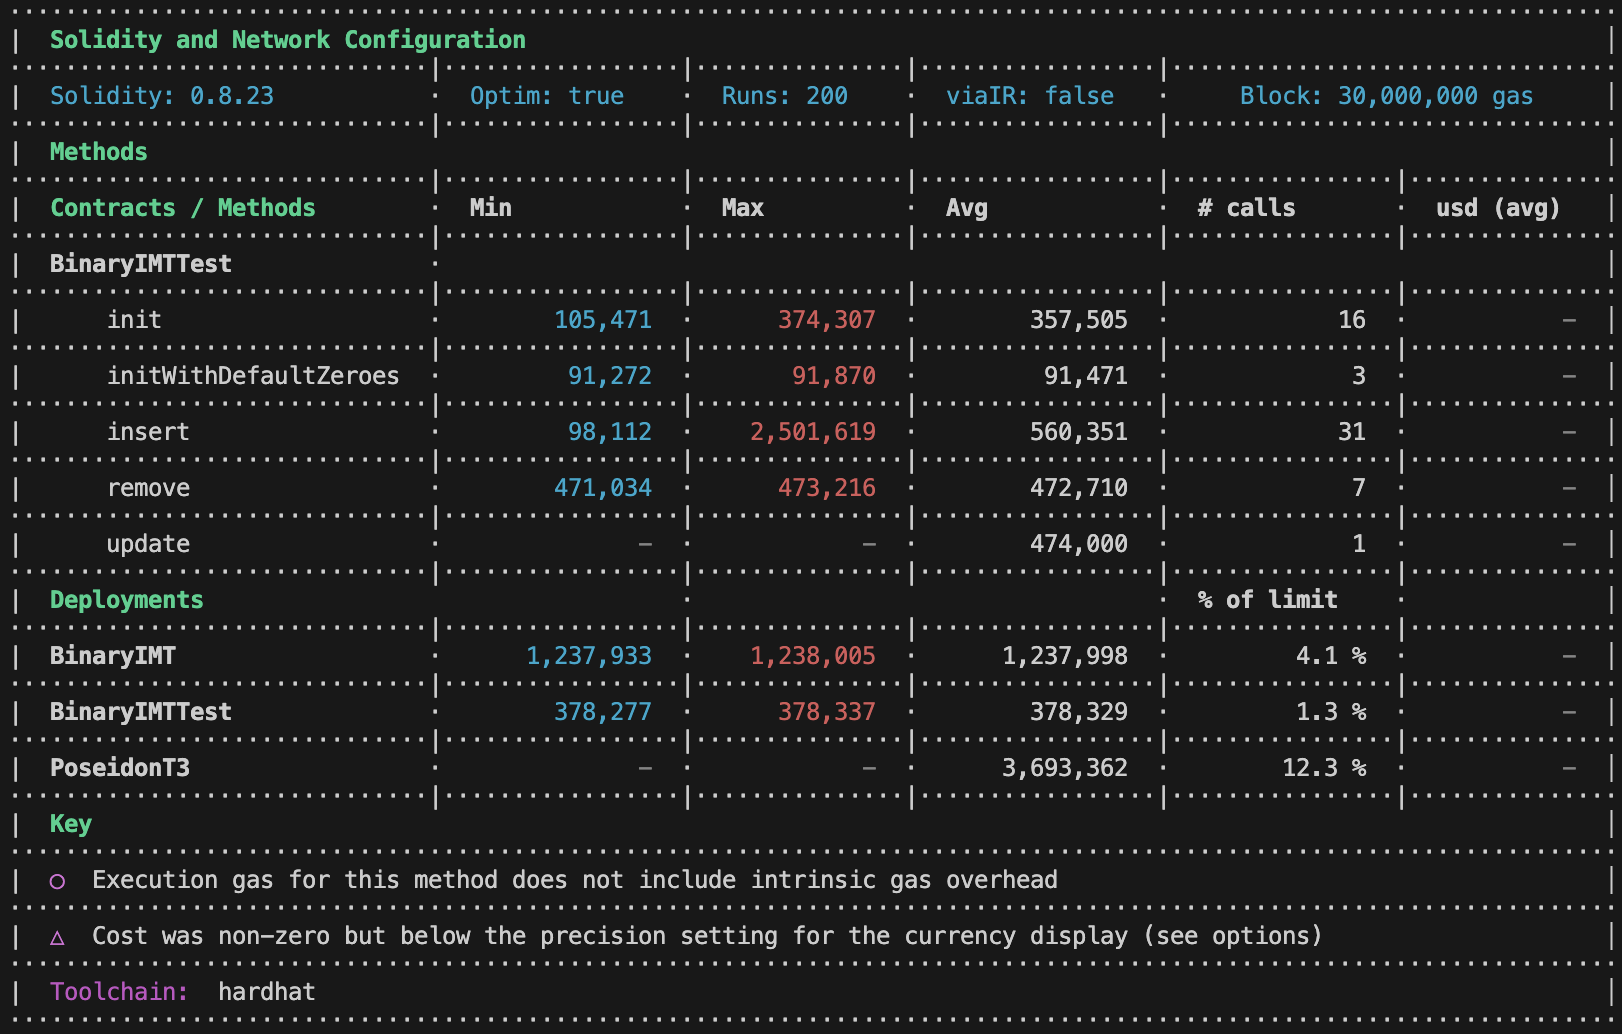
\includegraphics[width=\textwidth]{images/imt-gas-report.png}
    \caption{IMT Gas Report}
    \label{fig:imt-gas-report}
\end{figure}

\begin{figure}[H]
    \centering
    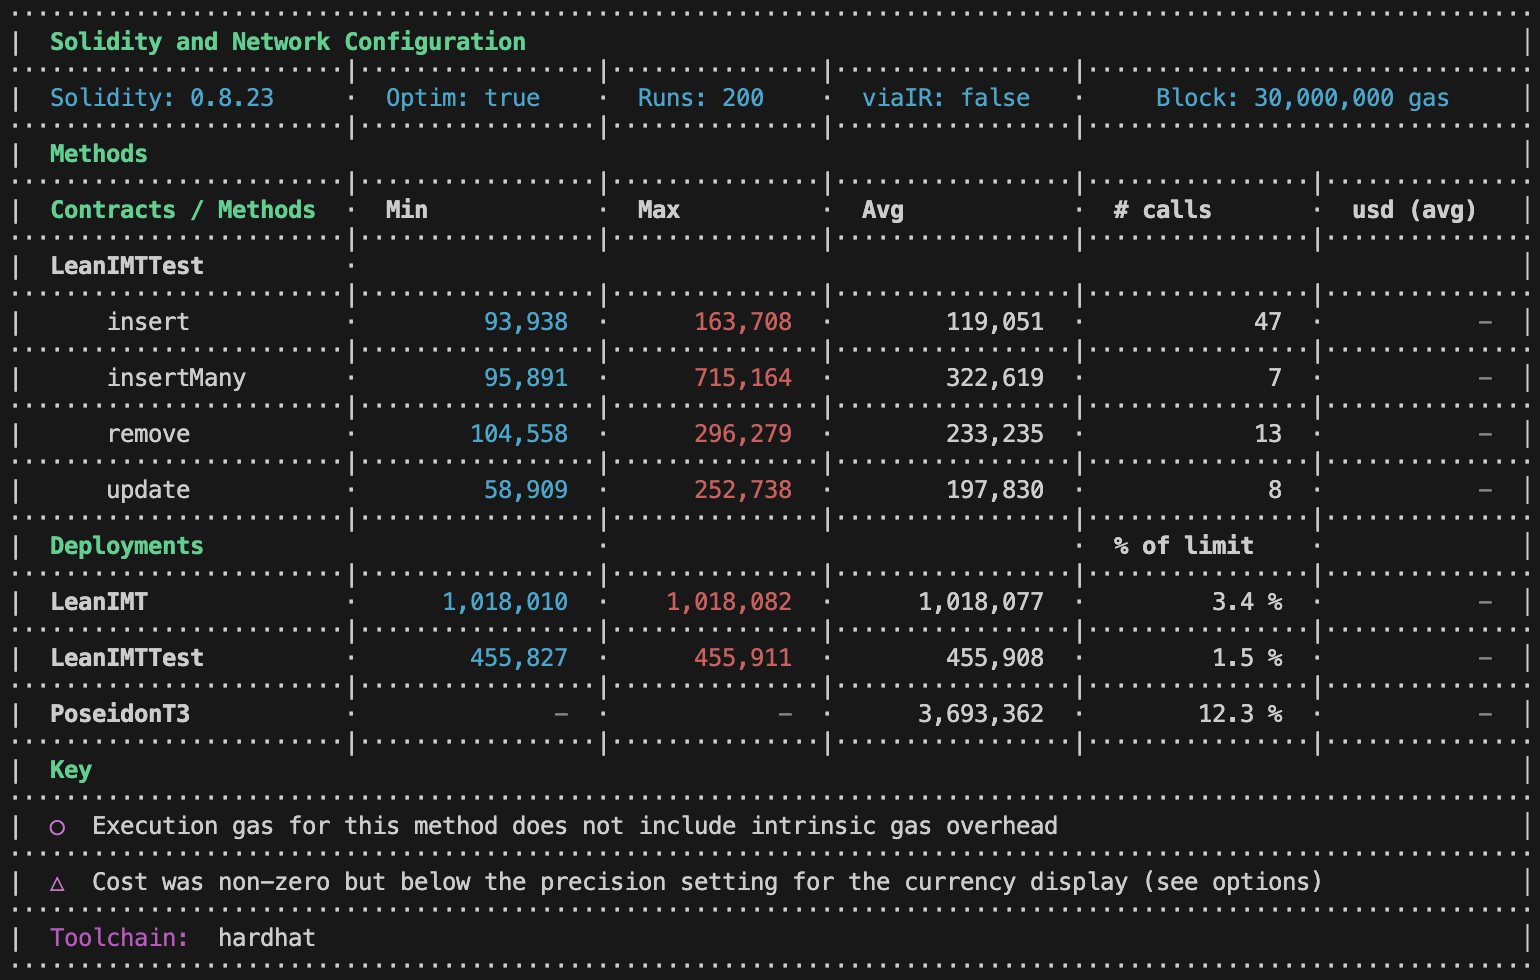
\includegraphics[width=\textwidth]{images/leanimt-gas-report.png}
    \caption{LeanIMT Gas Report}
    \label{fig:leanimt-gas-report}
\end{figure}

% Bar chart

\begin{figure}[H]
    \centering
    \pgfplotstableread[col sep=comma,]{data/gas-cost-functions-bar.csv}\datatable
    \begin{tikzpicture}
        \begin{axis}[
                ybar,
                xlabel={Function},
                xtick=data,
                xticklabels from table={\datatable}{Function},
                ylabel={Average Units of gas},
                ymin=0, % Set y-axis minimum to 0
                grid=major, % Add grid
                enlargelimits=0.15,
                legend style={at={(1.05,1)}, anchor=north west}, % Position the legend outside the plot
                legend cell align={left}, % Align legend text to the left
                % nodes near coords,
                xticklabel style={rotate=45, anchor=east} % Rotate x-axis labels
            ]
            \addplot[color=blue600, fill=blue400] table [x expr=\coordindex, y={IMT}, col sep=comma]{\datatable};
            \addlegendentry{IMT}

            \addplot[color=green600, fill=green400] table [x expr=\coordindex, y={LeanIMT}, col sep=comma]{\datatable};
            \addlegendentry{LeanIMT}
        \end{axis}
    \end{tikzpicture}
    \caption{Gas cost of the execution of the Functions IMT vs LeanIMT}
    \label{fig:gas-price-functions-bar}
\end{figure}

\section{Conclusionss}


% Example citation in the Introduction section
This document is based on the work of \cite{semaphorev1whitepaper}.

% Allow LaTeX to break lines more flexibly in the bibliography
\sloppy

% Bibliography section
\printbibliography

% This is the end of the document
\end{document}